\section{Objetivos y contextualización}

  Una práctica muy utilizada dentro del desarrollo de proyectos grandes de \textit{software} es el uso de testing unitario de los difernte componentes de la aplicación que sobre la que se trabaja. Esta práctica tiene dos objetivos principales: primero el poder tener seguridad de que el código escrito efectivamente cumple el propósito por el cuál fue programado, y en segundo lugar, el tener la seguridad de que al cambiar una parte del código, este siga cumpliendo su función original. En la práctica, el segundo punto es sumamente útil al momento de reazlizar cambios al \textit{code base} existente, dado que se quiere seguir teniendo la misma funcionalidad, pero cambiando el código interno, en lo que se conoce como \textit{refactor} y mediante las pruebas se puede tener la seguridad de que todo siga en orden después de haber realizado el o los cambios. 
  
  En este sentido, es paradójico que, una empresa que se dedica a producir \textit{software}, no haga pruebas de sus desarrollos internos. Es por lo anterior, que el alumno le sugirió a su superior, Nicolás Kipreos, aumentar significativamente la cantidad de pruebas que existen para el ERP, junto con la integración de estas a un flujo de integración continua de manera de que se pudiese tener una mayor seguridad y cofianza al momento de poner en producción el nuevo código.

  El pricipal beneficio que el área de \textit{TechOps} tendría mediante la implementación de una mayor cantidad de pruebas y la integración de estas pruebas a un flujo de integración continua serían tres. En primer lugar, el tener la seguridad de que el código efectivamente hace lo que se pretende que haga, en segundo lugar el saber que el código no se caerá de manera inesperada frente a un cambio y, en tercer lugar, el forzar a que el código sea probado antes de ser puesto en producción, evitando que los errores lleguen a los usuario de la plataforma.

  La meta que se estaableció por parte del alumno fue de llegar a una cobertura mínima de 60\% sin pruebas fallidas, junto con el forzar a que el flujo de \textit{deployment} de la aplicación fallara en caso que alguna prueba fallase en Circle CI.

\section{Desarrollo}

  En RoR, se hace uso de RSpec para hacer el \textit{testing} de manera automatizada y poder correr las pruebas correspondientes. En el caso de \textit{Hive}, cuando el alumno llegó al proyecto, este tenía una cobertura de 35,44\%. Esto quiere decir que solamente una de cada tres líneas de todo el código existente en \textit{Hive} era ejecutada y probada. Cabe mencionar también que aproximadamente un tercio de las pruebas que existían fallaban, es decir, el código no cumplía con las pruebas que se relizaban sobre el, teniendo un comportamiento diferente al esperado. En la figura \ref{fig:testing_original} se puede observa el estado inicial de la cobertura de las pruebas del ERP.

  \begin{figure}[H]
    \centering
    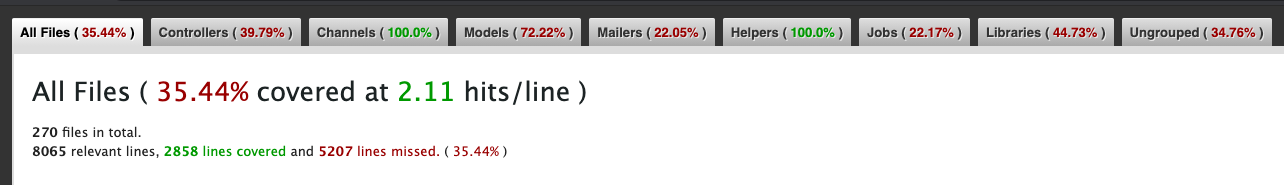
\includegraphics[width=\linewidth]{figures/testing/testing_original.png}
    \caption{Cobertura inicial del ERP (captura tomada el 3 de agosto de 2021).}
    \label{fig:testing_original}
  \end{figure}

  Dado que \textit{Hive}, en agosto, tenía aproximadamente 8000 líneas de código, el proceso del aumento de la cobertura del \textit{testing} comenzó mediante la revisión y mapeo de todos los archivos existentes y su estado de cobertura de pruebas. En otras palabras, se revisó todo el código fuente del ERP para saber cuáles archivos eran cubiertos por las pruebas automatizadas, cuáles no y cuáles requerían correcciones. De esta manera se podía ver con claridad en qué partes se tenía que enfocar los esfuerzos de trabajo y se podía saber cuáles archivo era más críticos de revisar y probar.

  El alumno realizó el mapeo de los archivos junto a Tomás Burotto y dejaron los registros en una sección especial de Jira. Esta documentación se organizó por secciones y subsecciones de archivos y carpetas, siguiendo la misma estructura de \textit{Hive}. Una vez que se transpasaron todos los archivos, se procedió a ponerles etiquetas del estado en que se encontraban, tal como se puede observar en la figura \ref{fig:mapeo_tests}.
  
  Se decidió tener 3 estados para la cobertura: ``\textit{complete}'', en el cual 100\% de las líneas correspondientes del archivo eran cubiertas, ``\textit{partial}'' y ``\textit{empty}''. Por otro lado, también existían 3 etiquetas para el estado en que se econtraban las pruebas: ``\textit{passing}'', ``\textit{failing}'' y ``\textit{skipped}''. Finalmente, se hizo una etiqueta adicional llamada ``\textit{missing}'' que se aplicó en el caso de que no existiese el archivo de pruebas correspondiente.
  

  \begin{figure}
    \centering
    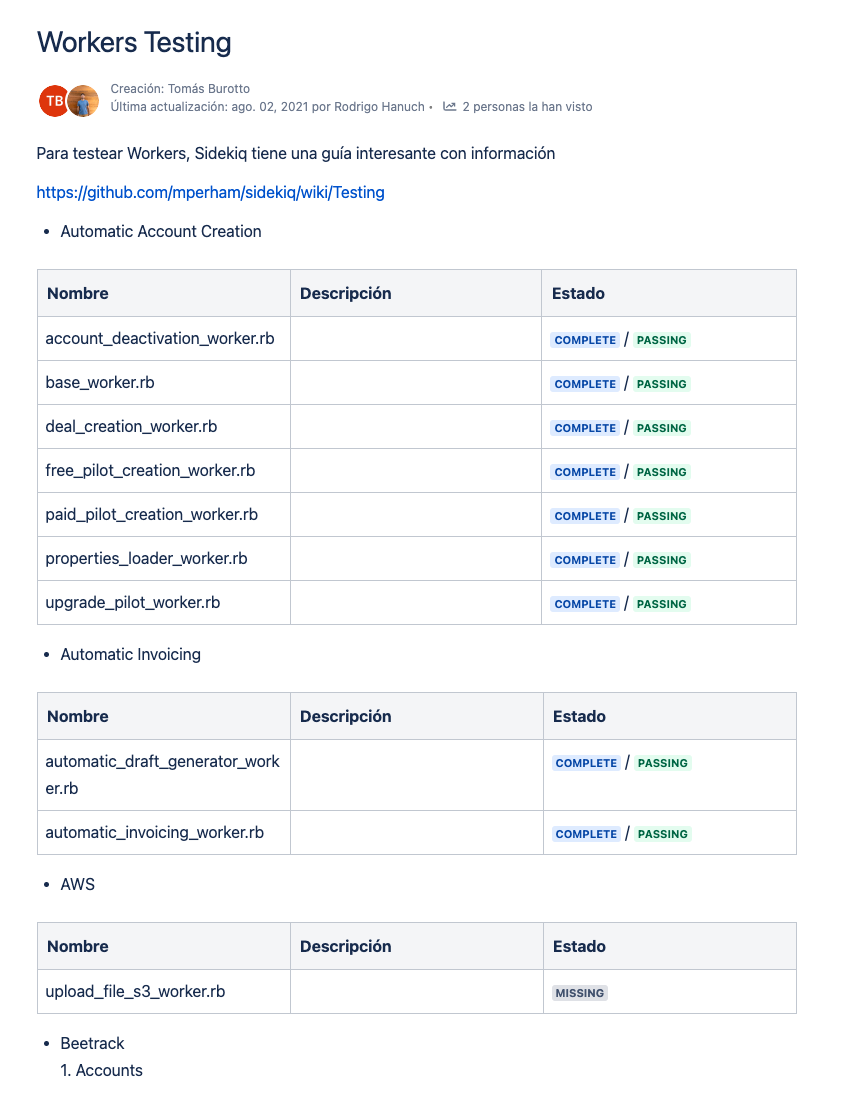
\includegraphics[width=0.75\linewidth]{figures/testing/mapeo_tests_existentes.png}
    \caption{Clasificación y etiquetado de los diferentes archvios y sus estados.}
    \label{fig:mapeo_tests}
  \end{figure}

\section{Resultados}